% Style based on 'Leap-Day' by Matt Graham:
%
%   https://github.com/mattgraham/Leap-Day
%
\documentclass{article}
\usepackage[a0paper]{geometry}
\usepackage{etoolbox}
\usepackage{xcolor}
\usepackage{graphicx}
%\usepackage{fontawesome}
\usepackage{tikz}
\usetikzlibrary{calc}

% fonts

\usepackage{lmodern}
\usepackage[T1]{fontenc}

% Fix small math symbols.
% source: http://tex.stackexchange.com/questions/74623/big-integral-in-lmodern
% TODO: Is there a better way to fix this?
\DeclareFontFamily{OMX}{lmex}{}
\DeclareFontShape{OMX}{lmex}{m}{n}{<-> lmex10}{}

\rmfamily

\renewcommand{\tiny}        {\fontsize{ 20.74pt}{ 25pt}\selectfont}
\renewcommand{\scriptsize}  {\fontsize{ 24.88pt}{ 30pt}\selectfont}
\renewcommand{\footnotesize}{\fontsize{ 29.86pt}{ 37pt}\selectfont}
\renewcommand{\small}       {\fontsize{ 35.83pt}{ 45pt}\selectfont}
\renewcommand{\normalsize}  {\fontsize{ 43.00pt}{ 54pt}\selectfont}
\renewcommand{\large}       {\fontsize{ 51.60pt}{ 64pt}\selectfont}
\renewcommand{\Large}       {\fontsize{ 61.92pt}{ 77pt}\selectfont}
\renewcommand{\LARGE}       {\fontsize{ 74.30pt}{ 93pt}\selectfont}
\renewcommand{\huge}        {\fontsize{ 89.16pt}{112pt}\selectfont}
\renewcommand{\Huge}        {\fontsize{107.00pt}{134pt}\selectfont}

\normalsize

% spaces

\setlength\parindent      { 2em}
\setlength\parskip        { 0pt plus .5ex}
\setlength\floatsep       {45pt plus  5pt minus  5pt}
\setlength\textfloatsep   {86pt plus  9pt minus 18pt}
\setlength\intextsep      {45pt plus  5pt minus 15pt}
\setlength\dblfloatsep    {45pt plus  5pt minus  5pt}
\setlength\dbltextfloatsep{86pt plus  9pt minus 18pt}

\setlength\abovedisplayskip     {32pt plus 3pt minus 3pt}
\setlength\abovedisplayshortskip{14pt plus 3pt minus 3pt}
\setlength\belowdisplayskip     {\abovedisplayskip}
\setlength\belowdisplayshortskip{\abovedisplayskip}

% list environments

\setlength\leftmargini  {2em}
\leftmargin  \leftmargini
\setlength\leftmarginii  {2.2em}
\setlength\leftmarginiii {1.87em}
\setlength\leftmarginiv  {1.7em}
\setlength\leftmarginv  {.5em}
\setlength\leftmarginvi {.5em}
\setlength  \labelsep  {.5em}
\setlength  \labelwidth{\leftmargini}
\addtolength\labelwidth{-\labelsep}
\makeatletter
\@beginparpenalty -\@lowpenalty
\@endparpenalty   -\@lowpenalty
\@itempenalty     -\@lowpenalty
\makeatother
\renewcommand\labelitemi{{\fontfamily{lmr}\selectfont\textbullet}}
\renewcommand\labelitemii{\normalfont\bfseries \textendash}
\renewcommand\labelitemiii{\textasteriskcentered}
\renewcommand\labelitemiv{\textperiodcentered}

% style lengths

\def\setnewlength#1#2{%
  \newlength{#1}%
  \setlength{#1}{#2}}

\setnewlength\safetymargin{3cm}
\setnewlength\headerheight{.2\paperwidth}
\setnewlength\headeryellowbarheight{.065\paperwidth}
\setnewlength\headeryellowbarlength{.8\paperwidth}
\setnewlength\footerheight{.1\paperwidth}
\setnewlength\footercontentheight{.6\footerheight}

% style colors

\definecolor{LDbackground}{HTML}{EAE6D1}
\definecolor{LDblue}{HTML}{4276B6}
\definecolor{LDyellow}{HTML}{FFCC00}
\definecolor{LDyellowborder}{HTML}{F0B500}
\definecolor{LDtextborder}{HTML}{CBCBCB}
\pagecolor{LDbackground}

% textbox

\def\textbox(#1) at (#2) [#3] <#4> #5{%
  \def\textboxname{#1}%
  \def\textboxpos{#2}%
  \def\textboxalign{#3}%
  \def\textboxwidth{#4}%
  \def\textboxtitle{#5}%
  \node[fill=white,draw=LDtextborder,inner sep=1em,shift={(0,-2em)},rounded corners=.5ex] (contents #1) at (#2) [#3] \bgroup%
    \begin{minipage}{#4}}%
\def\endtextbox{%
    \end{minipage}%
  \egroup;%
  \node[black,inner sep=0pt,shift={(1em,0.65em)}] at (contents \textboxname.north west) [above right] {%
    \large\sffamily\bfseries\textboxtitle};
}

% QR code

\ifx\directlua\undefined
  \def\qrcode<#1>[#2]#2{%
    \errmessage{qrcode: Please compile with `lualatex`.}}
\else
  \directlua{qrcode=dofile(kpse.find_file("qrcodehelper.lua"))}
  \def\hrefwrapper#1#2{% clickable link, only if `hyperref` package is loaded
    \ifcsdef{href}{%
      \href{#1}{#2}}{%
      #2}}
  \def\qrcode<#1>[#2]#3{%
    \bgroup%
      \newlength{\qrsize}%
      \setlength{\qrsize}{#1}%
      \def\qrcodecolor{#2}%
      \hrefwrapper{#3}{\directlua{qrcode.generate("\luaescapestring{#3}")}}%
    \egroup}
\fi

\pagestyle{empty}

\begin{document}%
\begin{tikzpicture}[remember picture,overlay,line width=.001\paperwidth]

% header

\fill[color=LDblue] ($(current page.north west)+(-\safetymargin,+\safetymargin)$) rectangle ($(current page.north east)+(+\safetymargin,-\headerheight)$);
\draw[color=LDyellowborder,fill=LDyellow,rounded corners=.5ex] ($(current page.north west)-(\safetymargin,\headerheight)+.5*(0cm,\headeryellowbarheight)$) rectangle ($(current page.north west)+(\headeryellowbarlength,-\headerheight)-.5*(0cm,\headeryellowbarheight)$);
\node[color=white] at ($(current page.north)-(0,.4\headerheight)$) {%
  \sffamily\bfseries\fontsize{100}{100}\selectfont%
  SIAM Student Chapter Delft};%
\node[color=white] at ($(current page.north)-(0,.65\headerheight)$) {%
  \sffamily\fontsize{60}{60}\selectfont%
  Delft University of Technology};
\node[color=black] at ($(current page.north west)-(-10.5*\safetymargin,\headerheight)$){%
  \sffamily\fontsize{45}{45}\selectfont%
  \textbf{Keywords:}  Applied Mathematics, Computer Science, Social Activities, Interdisciplinary Science.};
  
% footer

\newlength\footermargin
\setlength\footermargin{.5\footerheight}
\addtolength\footermargin{-.5\footercontentheight}

\draw[color=LDtextborder,fill=black!65] ($(current page.south west)+(-\safetymargin,-\safetymargin)$) rectangle ($(current page.south east)+(\safetymargin,\footerheight)$);
\node at ($(current page.south east)+.5*(-\footerheight,\footerheight)$) {
  \qrcode<\footercontentheight>[white]{http://sscdelft.github.io}};
\node [left,inner sep=0pt,white] at ($(current page.south east)+(-\footerheight,.5\footerheight)$) {%
  \ttfamily\fontsize{40}{45}\selectfont%
  \begin{tabular}{@{}r@{}}
    @SSC\_Delft\\
    siamsc-ewi@tudelft.nl\\
    http://sscdelft.github.io
  \end{tabular}};
\node [right,inner sep=0pt] at ($(current page.south west)+(0cm,.5\footerheight)$) {%
  \hspace{3\footermargin}%
  
\includegraphics[height=\footercontentheight]{tudelft}%
  \hspace{3\footermargin}%
  
\includegraphics[height=\footercontentheight]{siam}%
};

% content

\begin{textbox}(siam) at ($(current page.north west)+(3cm,-22cm)$) [below right] <45cm>
{Society for Industrial and Applied Mathematics}

  The \emph{Society for Industrial and Applied Mathematics (SIAM)} is an
  international community of over 13,000 individual members.  Almost 500
  academic, manufacturing, research and development, service and consulting
  organizations, government, and military organizations worldwide are
  institutional members. The goals are:

  \begin{itemize}
    \item To advance the {\color{LDblue}application of mathematics and computational
    science} to engineering, industry, science, and society.
    \item To {\color{LDblue}promote research} that will lead to effective new
    mathematical and computational methods and techniques for science,
    engineering, industry, and society.
    \item To {\color{LDblue}provide media for the exchange of information} and ideas
    among mathematicians, engineers, and scientists.
  \end{itemize}

\end{textbox}

\begin{textbox}(chapters) at ($(contents siam.south west)+(0cm,-2cm)$) [below right] <45cm>
{SIAM Student Chapters}

  A \emph{SIAM student chapter} resides at one or more colleges or
  universities, and ideally involves students and faculty members from
  different departments.  The purpose of a chapter is to generate interest in
  applied mathematics and computational science by providing students
  opportunities to:
  \begin{itemize}
    \item {\color{LDblue}Share ideas and enthusiasm} with fellow students and faculty
    from any relevant department on campus,
    \item Explore {\color{LDblue}career opportunities},
    \item Make {\color{LDblue}contacts} that will last a lifetime and to
    \item Develop {\color{LDblue}leadership skills}.
  \end{itemize}

\end{textbox}

\begin{textbox}(activities) at ($(contents chapters.south west)+(0cm,-1.8cm)$) [below right] <45cm>
{Chapter activities}
     \begin{tikzpicture}[overlay]
     \node at (39.5cm,2.8cm){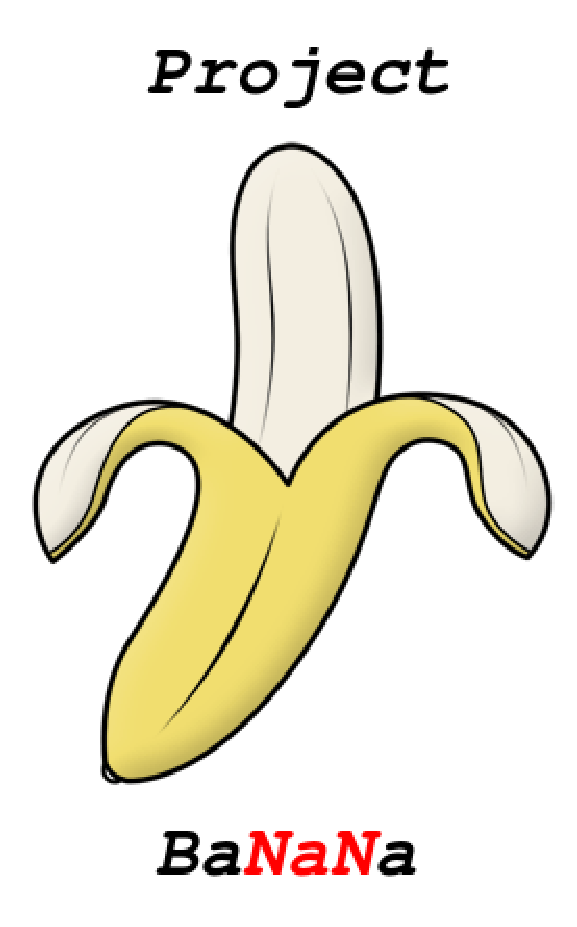
\includegraphics[scale=0.45]{baNaNa}};
    \end{tikzpicture}
  We are planing a couple of events:
  \begin{itemize}
    \item {\color{LDblue}Seminars and lectures} for and by PhD students,
    \item Student {\color{LDblue}Krylov day} at TU Delft on February 2, 2015,
    \item Learning-by-doing sessions on software tools [ba{\color{LDblue}NaN}a talks],
    \item {\color{LDblue}Socials events} like faculty BBQ, bowling, \dots
   \end{itemize}

\end{textbox}

\begin{textbox}(pictures) at ($(contents chapters.south west)+(0cm,-17.0cm)$) [below right] <75.3cm>
{}
 \includegraphics[height=9.5cm]{farm_golf} \hfill
 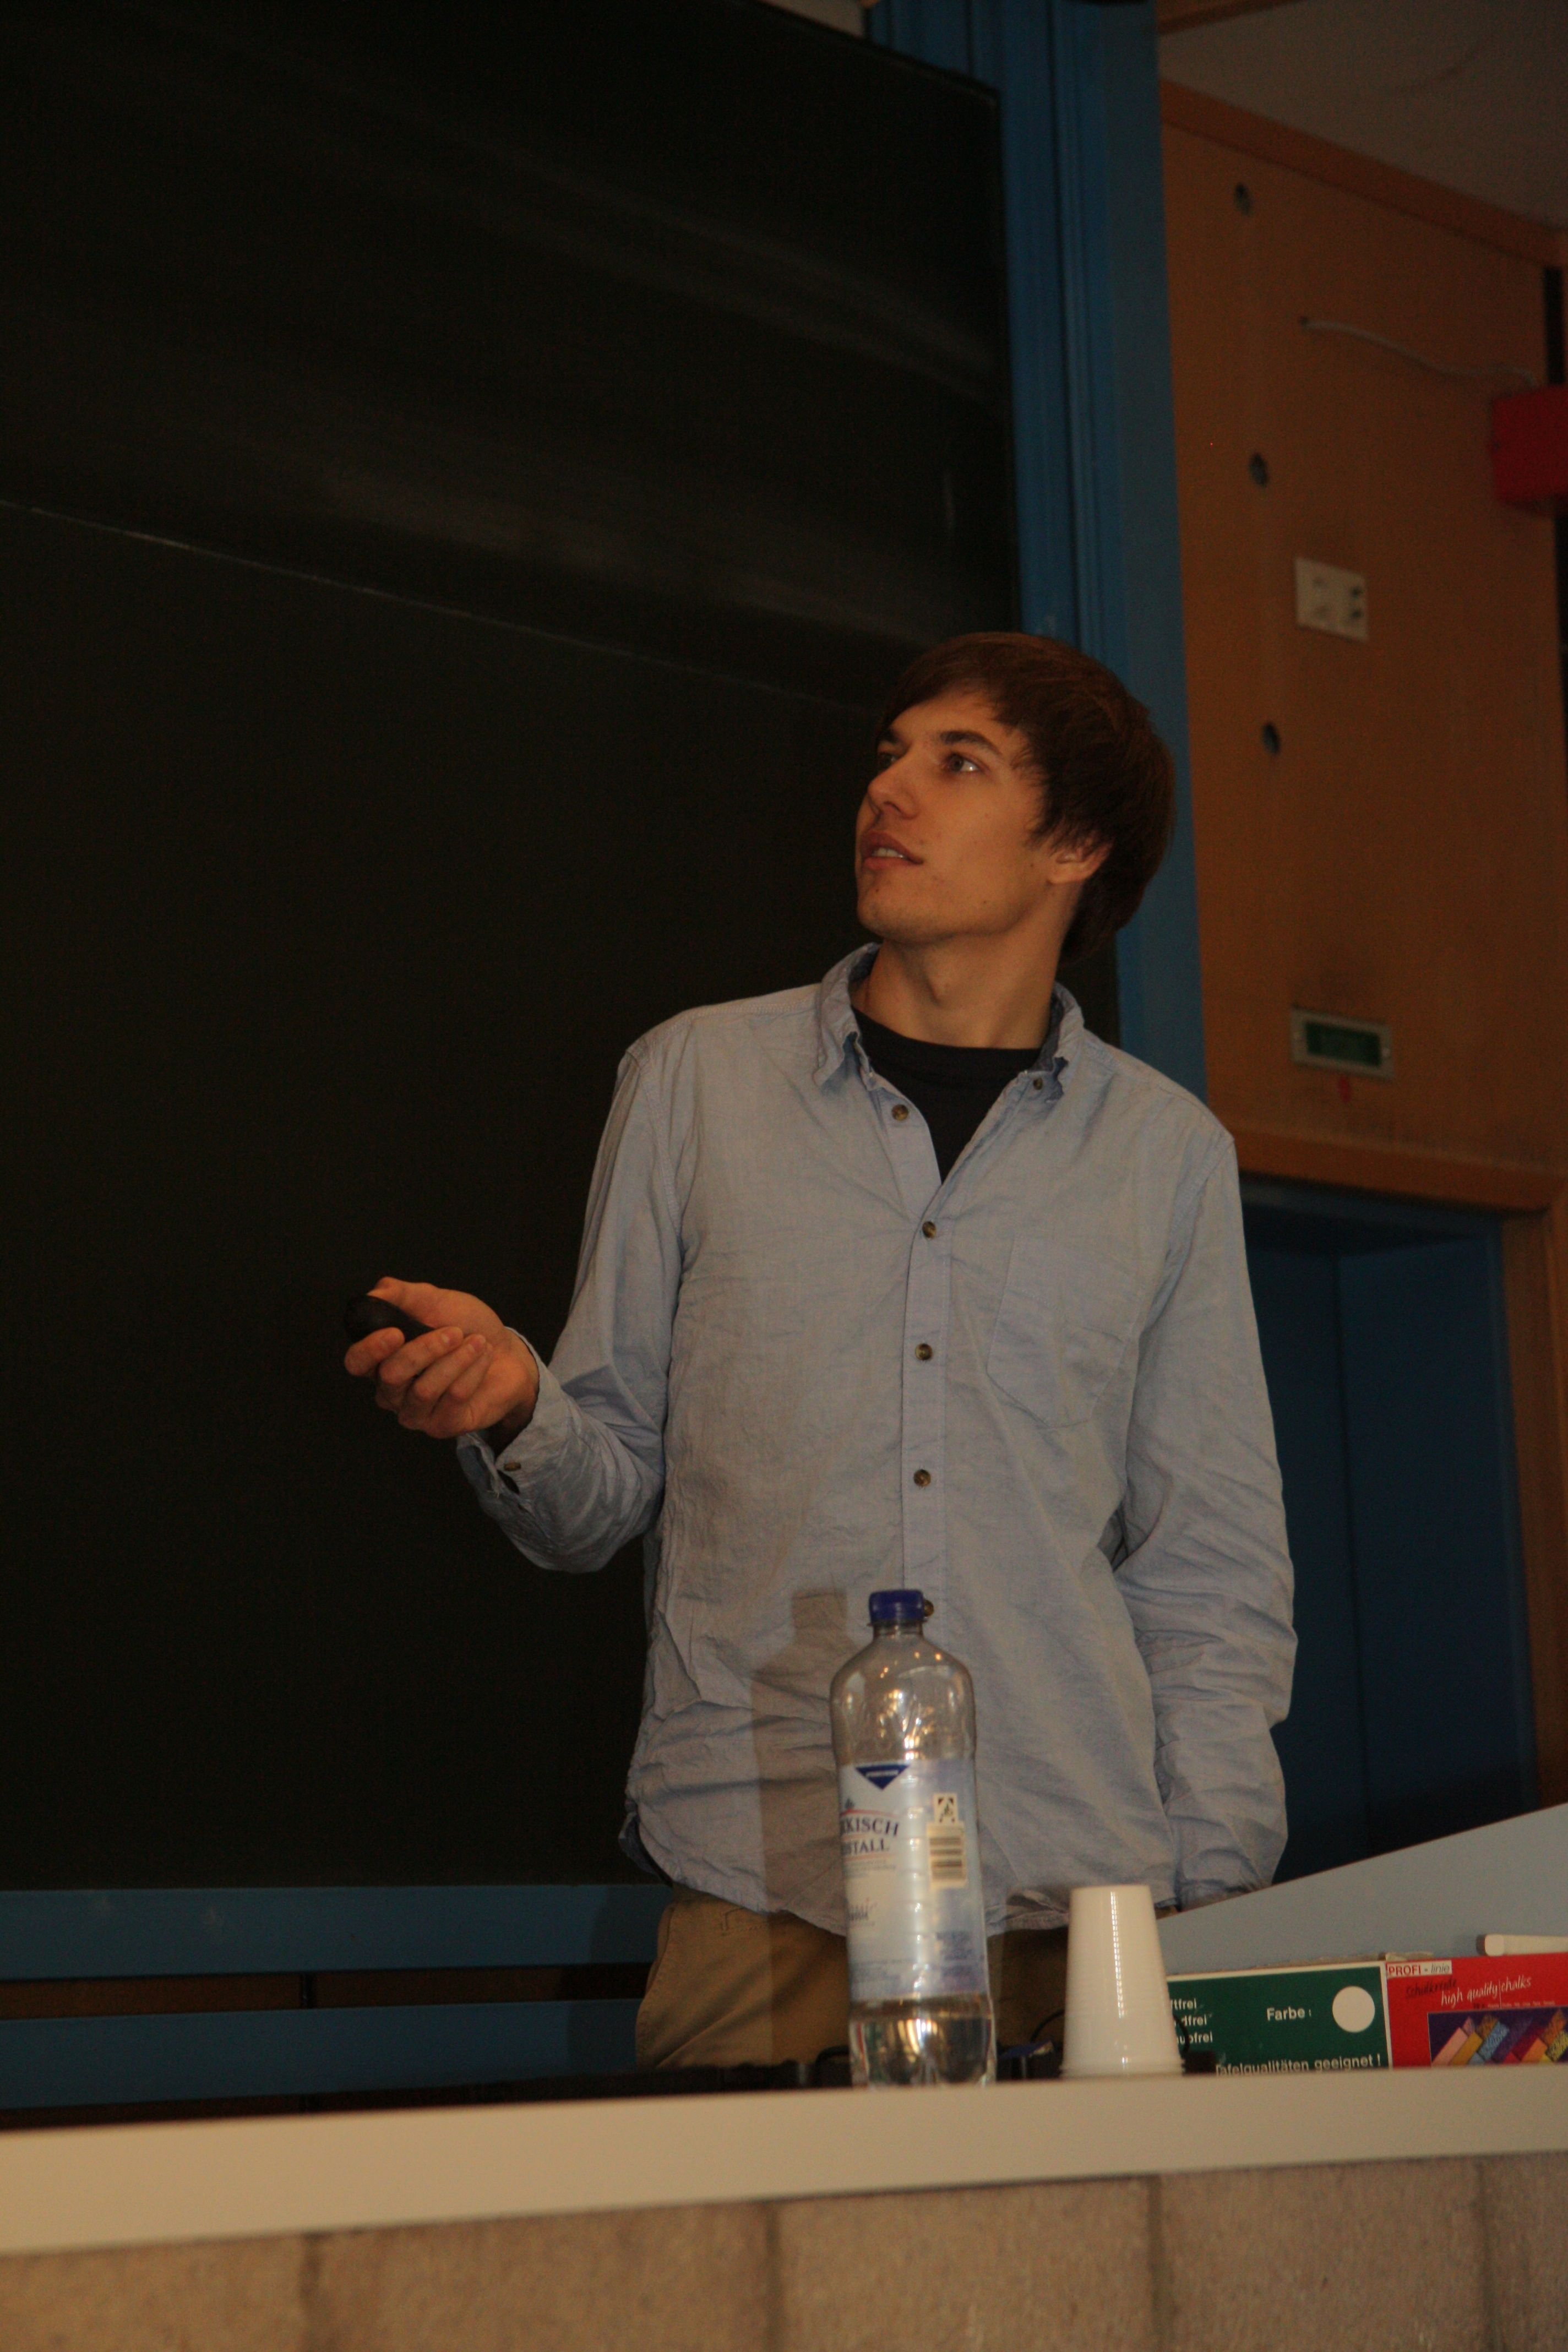
\includegraphics[height=9.5cm]{manuel_pres} \hfill
 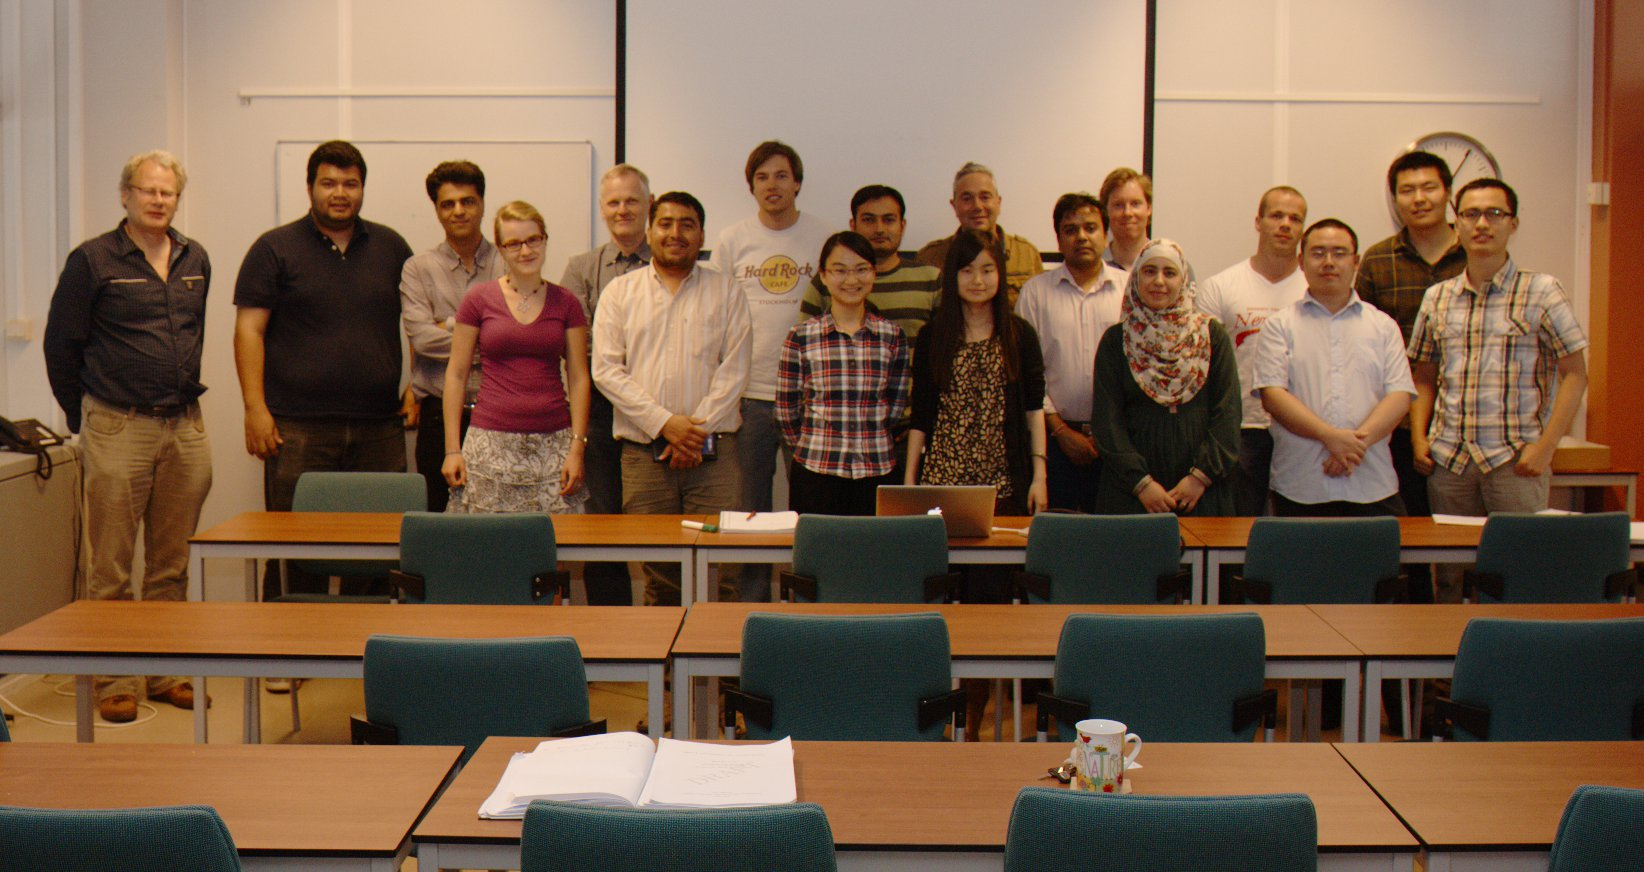
\includegraphics[height=9.5cm]{group} \hfill
 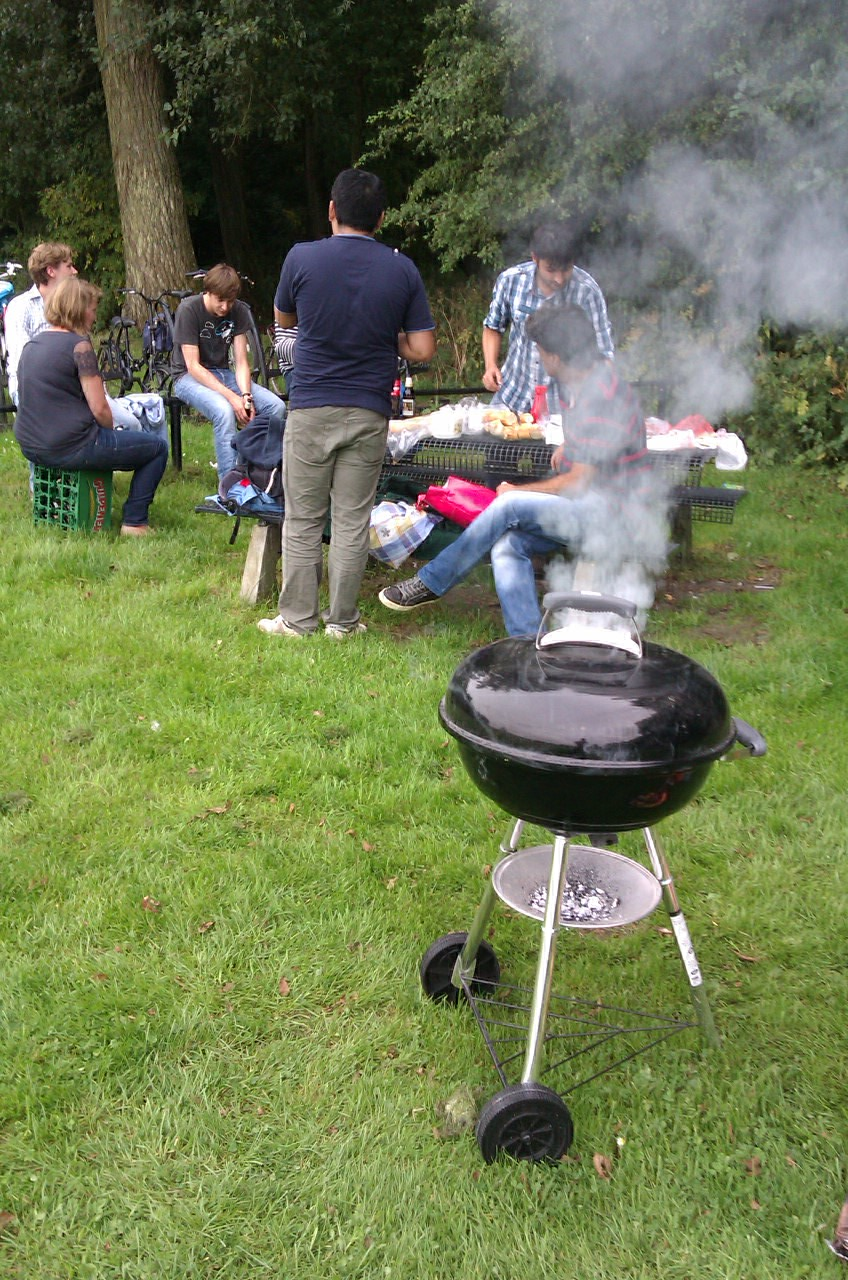
\includegraphics[height=9.5cm]{bbq} \hfill
 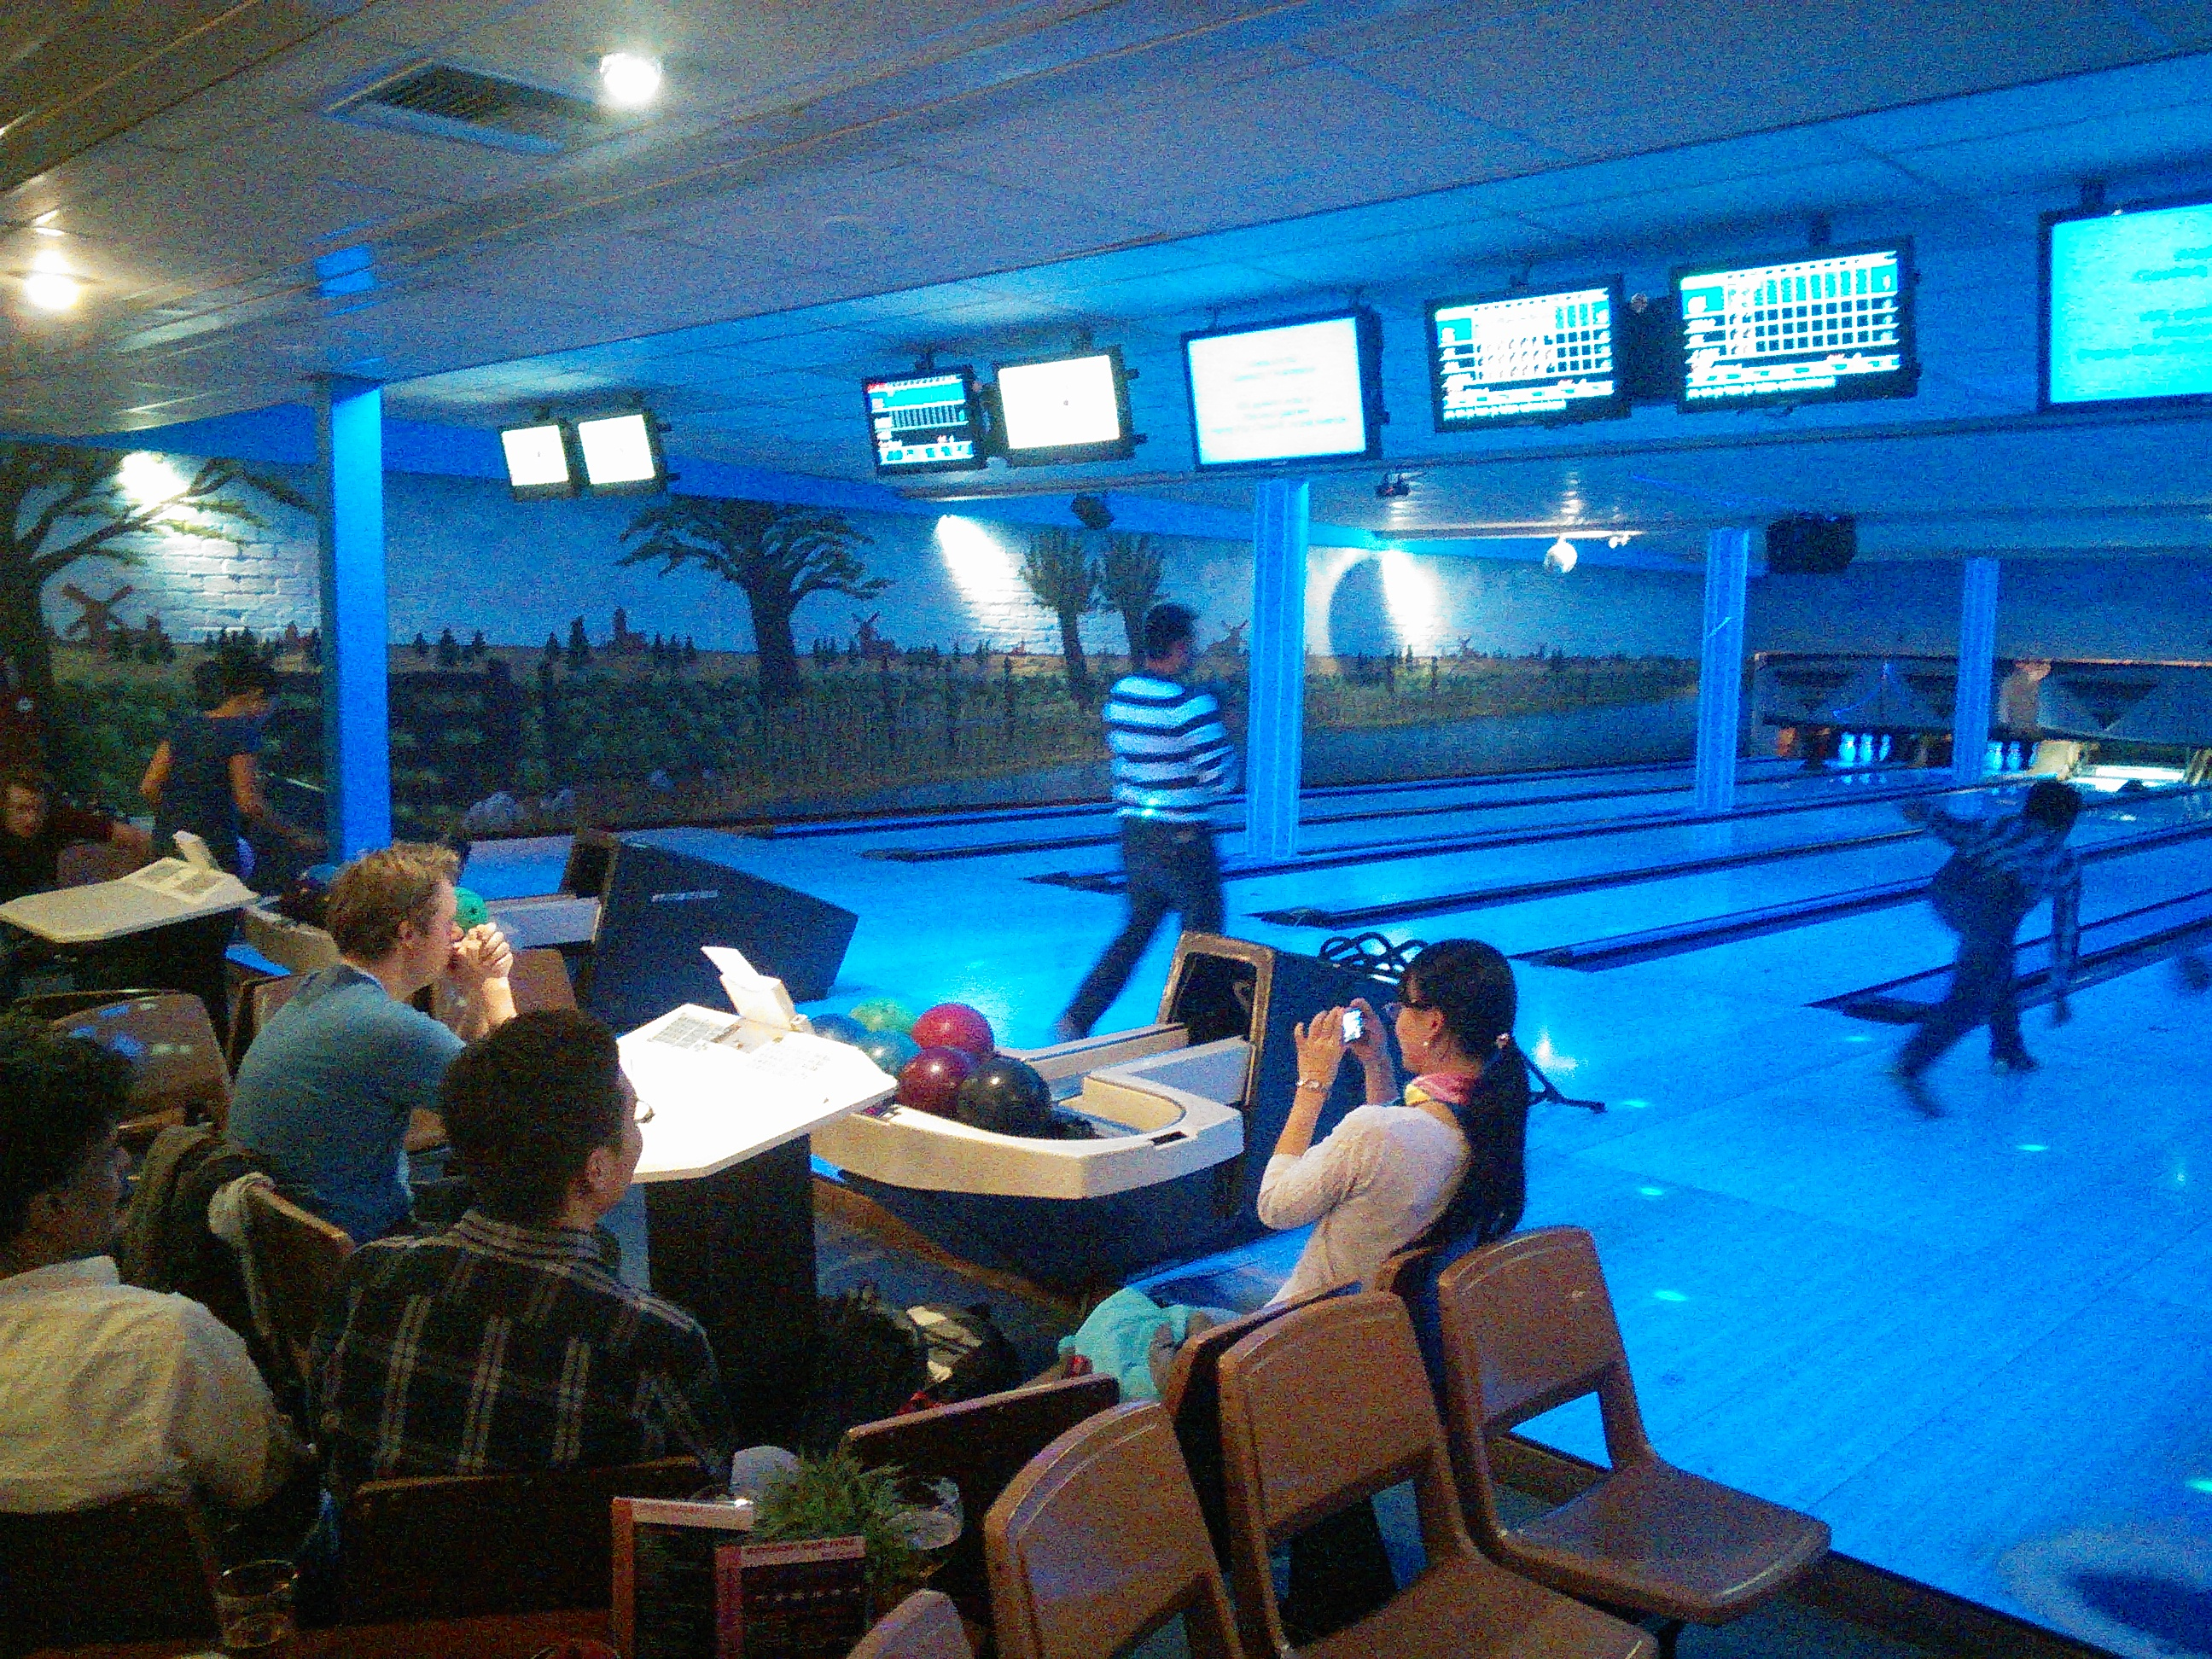
\includegraphics[height=9.5cm]{bowling} \hfill
 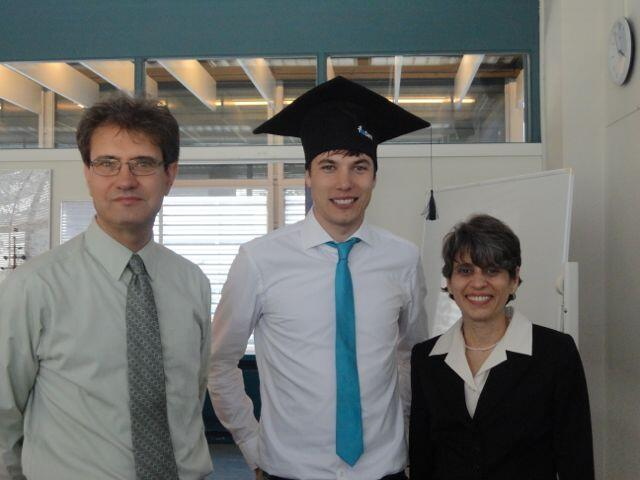
\includegraphics[height=9.5cm]{graduation}
\end{textbox}

\begin{textbox}(map) at ($(current page.north east)+(-3cm,-22cm)$) [below left] <24.4cm>
{SIAM chapters in Europe}

  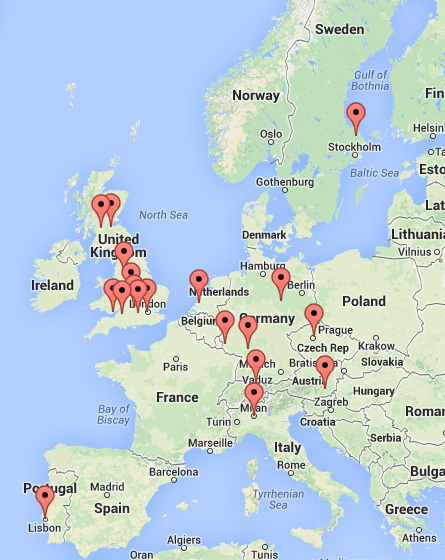
\includegraphics[width=\textwidth]{map}

  \begin{center}
    The first SIAM student chapter in the Netherlands is installed at TU Delft.
  \end{center}

\end{textbox}

\begin{textbox}(about) at ($(contents map.south east)+(0cm,-3cm)$) [below left] <24.4cm>
{Who are we?}

  The Chapter at TU Delft has been founded in 2014.

  \begin{itemize}
    \item \textbf{P:} Manuel Baumann
    \item \textbf{VP:} Reinaldo Astudillo
    \item \textbf{Sec. \& Treas.:} Thea Vuik
    \item ... and many more ;-)
  \end{itemize}

  Our faculty advisors are:
  \begin{itemize}
    \item Kees Vuik
    \item Martin van Gijzen
  \end{itemize}

  The Chapter is open for students and staff members.

\end{textbox}


\end{tikzpicture}%
\end{document}

% vim: ts=2:sts=2:sw=2:et
